\begin{center}
    \section{Семинар VI}
\end{center}
\subsection{Гармонический осциллятор в квантовой механике.}
Изучение гармонического осциллятора является настолько важным, потому что любое колебательное движение описывается гамильтонианом, аналогичным гамильтониану гармонического осциллятора. Этот семинар будет полностью посвящен особенностям описания колебательного движения в квантовой механике. Есть два подхода к описанию осциллятора в квантмехе: через непосредственное решение уравнения Шрёдингера и через операторы рождения и уничтожения. Я считаю второй подход более изящным и показательным, поэтому будем пользоваться именно им. Но сначала выполним несколько подготовительных действий. 

Во-первых, вспомним классическое описание гармонического осциллятора. Запишем его гамильтониан:
\[
H = \frac{p^2}{2M} + \frac{kx^2}{2}.
\]
Тогда уравнения движения будут иметь вид:
\[
\frac{dx}{dt} = \frac{p}{M}
\]
\[
\frac{dp}{dt} = -kx
\]
Найдя их решения и выразив частоту как $\omega = \sqrt{k/M}$, получим:
\[
x(t) = x(0)\cos\omega t + \frac{1}{M\omega}p(0)\sin\omega t
\]
\[
p(t) = p(0)\cos \omega t - M\omega x(0) \sin\omega t
\]

Во-вторых, перемасштабируем наблюдаемые координаты и импульса и сделаем их безразмерными. Для этого найдём коэффициенты A и B, где $\hat{X} = A\hat{x}$, $\hat{P} = B\hat{p}$, коммутатор этих наблюдаемых $\left[X, P \right] = i$  и эти наблюдаемые удовлетворяют уравнениям движения классического осциллятора:
\[
X(t) = X(0)\cos\omega t + P(0)\sin\omega t
\]
\[
P(t) = P(0)\cos \omega t - X(0) \sin\omega t
\]
Подставим в классические уравнения движения координату и импульс, выраженные через наши новые операторы $\hat{x} = \hat{X}/A\,\;\hat{p} = \hat{P}/B$:
\[
X(t) = X(0)\cos \omega t + \frac{1}{M\omega}\frac{A}{B}P(0)\sin\omega t;
\]
\[
P(t) = P(0)\cos \omega t - M\omega\frac{B}{A}X(0)\sin\omega t;
\]
Чтобы эти уравнения имели такой же вид, как и уравнения выше, необходимо чтобы
\[
\frac{A}{B} = M\omega
\]
Из коммутации же следует, что $\left[\hat{X}, \hat{P}\right] = AB\left[\hat{x},\hat{p}\right] = i\hbar AB$, т.е. $AB = \frac{1}{\hbar}$. Решая два полученных уравнения, находим
\[
A = \sqrt{\frac{M\omega}{\hbar}}; \; B = \frac{1}{\sqrt{M\omega \hbar}}
\]
Подставив их в выражения для операторов, получим
\[
\hat{X} = \sqrt{\frac{M\omega}{\hbar}}\hat{x}; \; \hat{P} = \frac{1}{\sqrt{M\omega \hbar}}\hat{p}
\]
Выпишу свойства этих операторов без вывода, так как их можно проверить самостоятельно:
\begin{itemize}
    \item $\bra{X}\ket{P} = \frac{1}{\sqrt{2\pi}}e^{iPX}$
    \item $\psi(X) = \left(\frac{\hbar}{M\omega}\right)^{1/4}\psi(x)$; $\;\psi(P) = \left(\hbar M\omega \right)^{1/4}\psi(p)$
    \item $\hat{P}\psi(X) = -i\frac{d}{dX}\psi(X)$;   $\;\hat{X}\psi(P) = i\frac{d}{dP}\psi(P)$
    \item $\langle\Delta X^2\rangle\langle\Delta P^2\rangle \geq \frac{1}{4}$
\end{itemize}
Гамильтониан же запишется как:
\[
\hat{H} = \frac{1}{2}\hbar\omega(\hat{X}^2 + \hat{P}^2)
\]
В-третьих, введём \textit{операторы рождения и уничтожения}. Оператор уничтожения определяется следующим образом:
\[
\hat{a} = \frac{1}{\sqrt{2}}\left(\hat{X} + i\hat{P} \right).
\]
Оператор рождения, в свою очередь, определяется как эрмитово сопряженный ему:
\[
\hat{a}^{\dagger} = \frac{1}{\sqrt{2}}\left(\hat{X} - i\hat{P} \right).
\]
Обратно, оператор координаты и импульса можно выразить как:
\[
\hat{X} = \frac{1}{\sqrt{2}}(\hat{a} + \hat{a}^{\dagger}); \;\; \hat{P} = \frac{1}{i\sqrt{2}}(\hat{a} - \hat{a}^{\dagger})
\]
Операторы рождения и уничтожения не коммутируют:
\[
[\hat{a}, \hat{a}^{\dagger}] = 1.
\]
Нам понадобится ещё одно коммутационное соотношение:
\[
[\hat{a}, \hat{a}^{\dagger}\hat{a}] = \hat{a}
\]
Теперь мы готовы обсудить квантовый гармонический осциллятор, его собственные значения и собственные состояния и особенности, которые отличают его от классического. Начнём с гамильтониана, записав его через операторы рождения и уничтожения:
\[
\hat{H} = \hbar\omega\left( \hat{a}^{\dagger}\hat{a} + \frac{1}{2}\right).
\]
Порядок операторов здесь очень важен. Именно оператор $\hat{a}^{\dagger}\hat{a}$ определяется как оператор числа квантов с собственным значением n и собственным состоянием $\ket{n}$. Такие состояния называются \textit{состояниями Фока}. Ясно, что собственные состояния и собственные значения гамильтониана будут такими же. Получается, что:
\[
\hat{a}^{\dagger}\hat{a}\ket{n} = n\ket{n}.
\]
Однако это не объясняет в полной мере, почему операторы имеют такое название. Давайте посмотрим на то, как операторы $\hat{a}$ и $\hat{a}^{\dagger}$ действуют на состояние $\ket{n}$. Для этого покажем, что состояние $\hat{a}\ket{n}$ является собственным для оператора $\hat{a}^{\dagger}\hat{a}$ с собственным значением $n-1$:
\[
\hat{a}^{\dagger}\hat{a}\hat{a}\ket{n} = (\hat{a}\hat{a}^{\dagger}\hat{a} - \hat{a})\ket{n} = (\hat{a}n - \hat{a})\ket{n} = (n-1)\hat{a}\ket{n}.
\]
Для оператора рождения аналогично:
\[
\hat{a}^{\dagger}\hat{a}\hat{a}^{\dagger}\ket{n} = (n+1)\hat{a}^{\dagger}\ket{n}.
\]
Мы все ещё не знаем, как действует оператор $\hat{a}$ на состояние $\ket{n}$, но теперь мы можем понять это из следующих рассуждений. Мы знаем, что энергетические спектры связанных состояний не вырождены, то есть каждому состоянию $\ket{n}$ соответствует только одно конкретное $n$. Тогда, так как собственное значение состояния $\hat{a}\ket{n}$ равно $n-1$, можно заключить, что состояние так же будет пропорционально $\ket{n-1}$. Почему пропорционально, а не равно? Потому что, в отличие от состояний $\hat{a}\ket{n}$ и $\hat{a}^{\dagger}\ket{n}$, состояния $\ket{n-1}$ и $\ket{n+1}$ нормированы по определению. Для первых же необходимо определить нормировочный коэффициент. Давайте сделаем это.

Пусть $\hat{a}\ket{n} = \ket{\phi}$. Мы знаем, что $\ket{\phi} = A\ket{n-1}$. Посчитаем двумя способами скалярное произведение введенного состояния на себя:
\[
\left[
\begin{gathered}
\bra{\psi}\ket{\psi} = \bra{n}\hat{a}^{\dagger}\hat{a}\ket{n} = n\\
\bra{\psi}\ket{\psi} = |A|^2\bra{n-1}\ket{n-1} = |A|^2
\end{gathered}
\right. => |A| = \sqrt{n}
\]
Сделав то же самое для оператора рождения, получим следующие уравнения:
\[
\hat{a}\ket{n} = \sqrt{n}\ket{n-1}
\]
\[
\hat{a}^{\dagger}\ket{n} = \sqrt{n+1}\ket{n+1}
\]
Теперь выбор названия этих операторов может стать чуть понятнее. Действительно, действие одного из этих операторов, например оператора уничтожения, на состояние с определенным количеством квантов энергии $E = \hbar\omega(n + 1/2)$ уменьшит количество квантов на единицу, и получится $E = \hbar\omega(n - 1/2)$. Получается, что, во-первых, количество уровней энергии в гармоническом осцилляторе дискретно, а во-вторых, эти уровни эквидистантны с расстоянием $\hbar\omega$, называемым квантом энергии. Получается, что мы представляем осциллятор как набор квазичастиц, количество которых определяет энергию системы. Такой подход (описание состояния системы через частицы и квазичастицы) называется \textit{вторичным квантованием}. Это очень элегантный метод, с которым вы познакомитесь более подробно на курсе статистической физики.

Вернёмся к осциллятору. Получается, с помощью оператора уничтожения мы можем понижать количество квантов. Но в какой-то момент энергия станет отрицательной, что не имеет смысла в нерелятивистской теории (с ситуациями, когда это возможно, мы познакомимся во втором семестре). Поэтому важно определить \textit{вакуумное состояние} $\ket{0}$. Определяется оно следующим образом:
\[
\hat{a}\ket{0} = \vec 0.
\]
Под нулём в правой части подразумевается нулевой вектор Гильбертового пространства. Понятно, что из вакуумного состояния можно получить любое состояние $\ket{n}$, используя оператор рождения:
\[
\ket{n} = \frac{(\hat{a}^{\dagger})^n}{\sqrt{n!}}\ket{0}
\]
Давайте посчитаем волновые функции вакуумных состояний в координатном представлении $\bra{X}\ket{0}$ и затем обобщим это на произвольное фоковское состояние $\ket{n}$:
\[
\hat{a}\ket{0} = (\hat{X} + i\hat{P})\ket{0} = 0
\]
Умножим слева на бра состояние $\bra{X}$:
\[
\bra{X}\hat{X}\ket{0} + i\bra{X}\hat{P}\ket{0} = (X + \frac{d}{dX})\psi(X) = 0
\]
Решением этого обыкновенного дифференциального уравнения будет функция $\psi(X) = Ae^{-X^2/2}$. Вычислим коэффициент A из условия нормировки:
\[
\braket{\psi} = \int |\psi(X)|^2 dX = |A|^2\int e^{-X^2}dX = |A|^2\sqrt{\pi}
\]
В итоге получаем:
\[
\psi_0(X) = \frac{1}{\pi^{1/4}}e^{-X^2/2}
\]
В общем случае волновая функция будет выглядеть следующим образом:
\[
\psi_n(X) = \frac{H_n(X)}{\pi^{1/4}\sqrt{2^n n!}}e^{-X^2/2}, \text{где } H_n(X) = (X - \frac{d}{dX})^n - \text{полиномы эрмита}.
\]
Теперь немного обсудим результаты, которые получили. Для начала заметим, что в вакуумном состоянии импульс и координата неопределенны. Это называется \textit{Нулевыми колебаниями} – в состоянии минимальной энергии мы обнаруживаем отклонение от положения равновесия. То же самое со скоростью. Это отличает квантовый осциллятор от классического. Далее, волновые функции фоковских состояний, в отличие от потенциальных ям, которые мы рассматривали на прошлых семинарах, не кусочно определены, а представляют собой единые элементарные функции. Количество пересечений с осью абсцисс равно числу квантов n (рис. \ref{fig 6.8}). 
\begin{figure}[!ht]
\centering
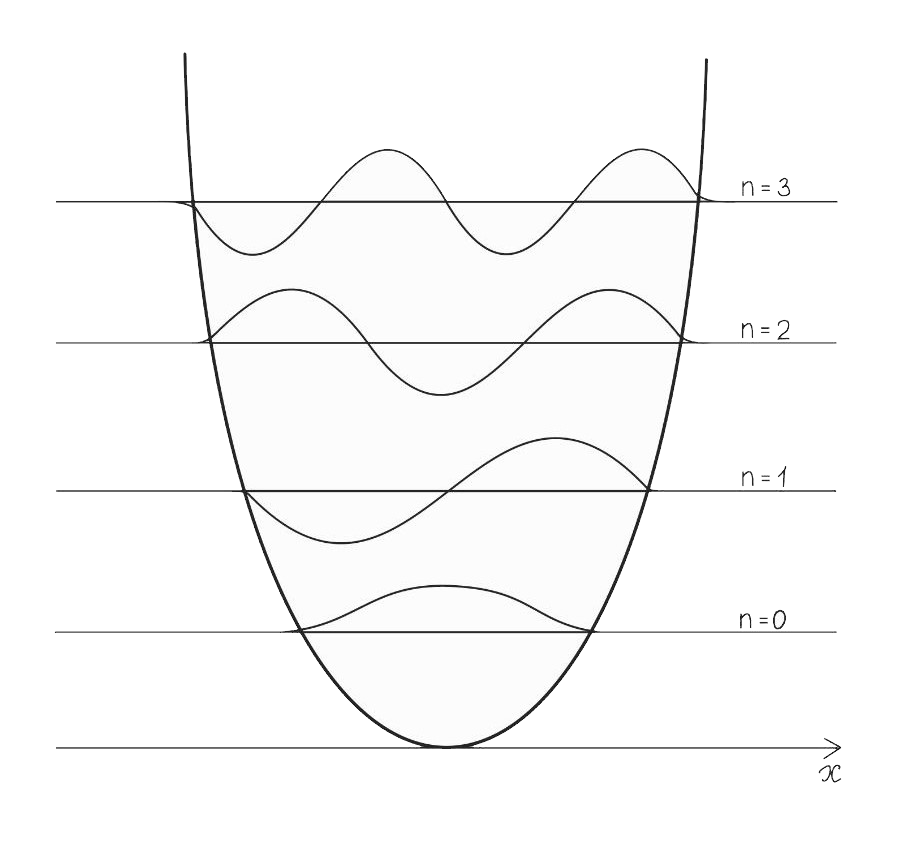
\includegraphics[scale=0.4]{class_6/images/oscillator.png}
\caption{Первые несколько уровней квантового гармонического осциллятора.}
\label{fig 6.8}
\end{figure}
\newpage
Может возникнуть вопрос: чему равны собственные состояния для оператора $\hat{a}$ или $\hat{a}^{\dagger}$ (напомню, что состояния $\ket{n}$ собственные для оператора $\hat{a}^{\dagger}\hat{a}$)? Оказывается, что такие состояния называются когерентными. Они играют большую роль в описании физических систем, так как в когерентном состоянии неопределенность минимальная – значит оно максимально приближает классический осциллятор. Мы не будем обсуждать когерентные состояния подробнее, так как они не присутствует в задачах, однако настоятельно рекомендую прочитать про эту тему самостоятельно. Мы переходим к решению задач на осциллятор.


\excersize{Упражнение №21}{darklavender}
\begin{center}
    \textit{Воспользовавшись повышающим и понижающим операторами $\hat a^+$ и $\hat a$, найдите средние значения оператора $\hat x^2,\,
    \hat x^4$ и $\hat x^{2k+1}$ в $n$-м стационарном состоянии линейного гармонического осциллятора.}
\end{center}
Давайте вспомним из теории, как выглядит оператор координаты $\hat X$: 
\[
\hat x = \frac{x_0}{\sqrt{2}}(\hat a^{\dagger} + \hat a),\quad x_0 = \sqrt{\frac{\hbar}{m\omega}}
\]
Тогда, запишем среднее значение по определению и, используя действия оператора рождения и оператора уничтожения на энергетический уровень n ($\hat a\ket{n} = \sqrt{n}\ket{n-1}$ и $\hat{a}^{\dagger}\ket{n} = \sqrt{n+1}\ket{n+1}$) посчитаем:
\begin{multline*}
    \bra{n}\hat x^2 \ket{n} = \frac{x^2_0}{2}\bra{n}(\hat a^{\dagger} + \hat a)^2\ket{n} = \frac{x^2_0}{2}(\bra{n}\hat a^{\dagger}\hat a^{\dagger}\ket{n} +\bra{n}\hat a\hat a\ket{n} + \bra{n}\hat a^{\dagger}\hat a\ket{n} + \bra{n}\hat a\hat a^{\dagger}\ket{n}) =\\
    \frac{x^2_0}{2}(\sqrt{(n+1)(n+2)}\bra{n}\ket{n+2} + \sqrt{(n)(n-1)}\bra{n}\ket{n-2} + \sqrt{(n+1)(n+1)}\bra{n}\ket{n} + \sqrt{(n) (n)}\bra{n}\ket{n})
\end{multline*}
Мы знаем, что вектора различных уровней ортогональны, а значит все скалярные произведения для различных n будут равны 0. Тогда останется следующее:
\[
\bra{n}\hat x^2\ket{n} = \frac{x^2_0}{2}((n+1) + n) = x^2_0(n + \frac{1}{2})
\]
Поступая точно так же с четвертой степенью, получим:
\[
\bra{n}\hat x^4\ket{n} = \frac{x_0^4}{4}(6n^2 + 6n + 3)
\]
Теперь с нечетной степенью. Достаточно заметить, что в случае разложения по нечетным степеням, у нас не будет членов с последовательными действиями операторов с одинаковыми степенями ($\hat a\hat a^{\dagger},\; \hat a\hat a^{\dagger}\hat a\hat a^{\dagger}$ и т.п.). Тогда все скалярные произведения будут равны нулю. Значит: 
\[
\bra{n}\hat x^{2k+1}\ket{n} = 0
\]
\csquare{darklavender}
\excersize{Упражнение №22}{darklavender}
\begin{center}
    \textit{Частица массы $m$ движется в потенциале трехмерного изотропного осциллятора:}
    \[
    U(r) = \frac{m\omega^2r^2}{2}.
    \]
    \textit{Найдите энергии уровней, кратности их вырождения, а также волновые функции стационарных состояний, разделяя переменные: а) в декартовых координатах, б) в сферических координатах. Обсудите связь задачи с моделью ядерных оболочек и получите первые магические числа: 2, 8, 20.}

    \textit{Определите четности стационарных состояний. Может ли осциллятор, находящийся в состоянии с определенной энергией, обладать отличным от нуля электрическим дипольным моментом (см. задачу 1)?}
\end{center}
В этом семинаре решим только в декартовых координатах. В следующих семинаре, когда пройдём движение в центральном поле, решим в сферических координатах.

Давайте подставим потенциал в уравнение Шрёдингера:
\[
-\frac{\hbar^2}{2m}\Delta\psi(\vec{r}) + \frac{m\omega^2\vec{r}^2}{2}\psi(\vec{r}) = E\psi(\vec{r})
\]
Так как координаты декартовы, можем записать Гамильтониан в виде:
\[
\hat H = \sum\limits_{i=1}^3(-\frac{\hbar^2}{2m}\frac{\partial^2}{\partial x_i^2} + \frac{m\omega^2x_i^2}{2})
\]
Такой гамильтониан коммутирует с каждым из операторов координаты $\hat{x}, \hat{y}, \hat{z}$, а значит решение можно искать в виде произведения их собственных функций. В то же время, это гамильтониан гармонического осциллятора, т.е. его можно описать через оператор $\hat{a}^{\dagger}\hat{a}$. Тогда эти функции будут ещё и собственные для этого оператора. В итоге можем записать волновые функции в следующем виде:
\[
\psi_{n_1n_2n_3}(\vec{r}) = u_{n1}(X)u_{n2}(Y)u_{n3}(Z)
\]
\[
u_{n_i}(X_i) = \frac{1}{\pi^{\frac{1}{4}}\sqrt{2^{n_i}n_i!}}e^{-X^2/2}H_{n_i}(X)
\]
где $H_{n}(X)$ - полиномы Эрмита. Энергия тогда будет иметь вид:
\[
E_n = \hbar\omega(n+\frac{3}{2}), \text{ где } n = n_1 + n_2 + n_3
\]
Давайте посчитаем кратность вырождения уровней. Если мы произвольно задаём $n_1 \leq n$, то тогда для $n_2$ останется $n-n_1+1$ вариантов ($n_2 = 0, 1, ... ,n - n1$). В этом случае $n_3 = n - n_1 - n_2$ зафиксировано, и можно посчитать кратность вырождения, используя формулу арифметической прогрессии: 
\[
\sum\limits_{n_1 = 0}^n n_2 = \sum\limits_{n_1 = 0}^n n-n_1 + 1 = \frac{1}{2}(n+1)(n+2)
\]
Посмотри, что получилось. Если n = 0, то кратность вырождения 1, то есть в стационарном состоянии у нас нет вырождения по координате. Если n = 1, то кратность вырождения 3, то есть на втором уровне у нас три возможных состояний координаты с одинаковым состоянием энергии. Если проследить последовательность, то можно заметить, что это очень сильно напоминает расположение электронов на оболочке атома (без учёта вырождения по спину). И это не просто так! Далее мы увидим, что осциллятором вполне можно приблизить модель атомной оболочки.
\csquare{darklavender}

В следующем семинаре мы обсудим движение в центральном поле и спин.

